%%%%%%%%%%%%%%%%%%%%%%%%%%%%%%%%%%%%%%%%%%%%%%%%%%%%%%%%%%%%%%%%%%
%%%%%%%% ICML 2014 EXAMPLE LATEX SUBMISSION FILE %%%%%%%%%%%%%%%%%
%%%%%%%%%%%%%%%%%%%%%%%%%%%%%%%%%%%%%%%%%%%%%%%%%%%%%%%%%%%%%%%%%%

% Use the following line _only_ if you're still using LaTeX 2.09.
%\documentstyle[icml2014,epsf,natbib]{article}
% If you rely on Latex2e packages, like most moden people use this:
\documentclass{article}

% use Times
\usepackage{times}
% For figures
\usepackage{graphicx} % more modern
%\usepackage{epsfig} % less modern
\usepackage{subfigure} 

% For citations
\usepackage{natbib}

% For algorithms
\usepackage{algorithm}
\usepackage{algorithmic}

% As of 2011, we use the hyperref package to produce hyperlinks in the
% resulting PDF.  If this breaks your system, please commend out the
% following usepackage line and replace \usepackage{icml2014} with
% \usepackage[nohyperref]{icml2014} above.
\usepackage{hyperref}

% Packages hyperref and algorithmic misbehave sometimes.  We can fix
% this with the following command.
\newcommand{\theHalgorithm}{\arabic{algorithm}}

%USER defined Packages
\usepackage{amsmath}


% Employ the following version of the ``usepackage'' statement for
% submitting the draft version of the paper for review.  This will set
% the note in the first column to ``Under review.  Do not distribute.''
%\usepackage{icml2014} 
% Employ this version of the ``usepackage'' statement after the paper has
% been accepted, when creating the final version.  This will set the
% note in the first column to ``Proceedings of the...''
\usepackage[accepted]{icml2014}


% The \icmltitle you define below is probably too long as a header.
% Therefore, a short form for the running title is supplied here:
\icmltitlerunning{Video Segmentation as a Distributed Convex Problem}

\begin{document} 

\twocolumn[
\icmltitle{Video Segmentation as a Distributed Convex Optimization Problem\\
 using Primal Decomposition} 

% It is OKAY to include author information, even for blind
% submissions: the style file will automatically remove it for you
% unless you've provided the [accepted] option to the icml2014
% package.
\icmlauthor{Animesh Garg*}{animesh.garg@berkeley.edu}
\icmlauthor{Jeff Mahler*}{jmahler@berkeley.edu}
\icmlauthor{Shubham Tulsiani*}{shubhtuls@berkeley.edu}
\icmladdress{Department of EECS, UC Berkeley, CA 94720}

% You may provide any keywords that you 
% find helpful for describing your paper; these are used to populate 
% the "keywords" metadata in the PDF but will not be shown in the document
\icmlkeywords{Tracking, Segmentation, Video, Convex Optimization, Subgradient Learning}

\vskip 0.3in
]

\begin{abstract} 
Getting exact video segmentations for tracking and recognition is a challenging problem. 
A majority of existing methodstrack but provide a bounding box rather than a an exact foreground
mask for the object. For real worl applications of perception, like robotics, the silhoutte of the object
perhaps even pose need to be known for hope of success in manipulation tasks.

We propose a method in this study which formulated the problem of video segmentation
as a Markov random field. However solving such a large graph to global optimality may 
be computationally expensive. Hence we propose a distributed method using Primal 
decomposition. 

\end{abstract} 

\section{Introduction}

The problem of video segmentation is of interest for many areas. 
\cite{Komodakis2007a, Komodakis2011a} and \cite{Tsai2010}
have looked at the problem of modelling the MRF in terms of energies. 
The solution strategy they use is Dual decomposition but without integer programming.

Our study explores the use of state-of-the-art integer program solvers. Modelling integers
allows us to capture more rich features in video which are usually not directly put in current 
models. 
From a given video sequence, and user intialized object(s)
of interest, the aim is to track the region(s) of interest through
the subsequent image frames in the video. Majority of other
methods which address the problem provide locally optimal
solutions. Such an approach though successful in some applications
requires a substantial amount of human intervention
at several points in the solution such as in cases of occlusion,
change in pose, shape and color and in extreme cases object
(or a part of object) egresses the frame and re-enters later.

\section{Related Work}

Automatic video segmentation has been studied and solutions mostly provide a 
bounding box track. However several applications require a higher fidelity 
track to accurately localize the foreground in the video. This problem is of 
importance in several areas of research like behavior analysis in animal studies and object tracking for robot perception, among others.  The problem of foreground tracking and more generally, the problem of video segmentation are well studied in the field of Computer Vision. Many of the prominent approaches treat the problem of video segmentation as that of combining segments obtained independently for various frames. 

A standard approach is to leverage standard image segmentation algorithms like \cite{CPMC} and filter the segmentation candidates to ensure consistency accross frames. Another commonly used approach where the generated segmentations rely on temporal information is to incorporate the optical flow information of the frame along with the intensity as an additional layer image and use segmentation algorithms for this layered image eg \cite{LeordeanuSS12}. We observe that these common methods either do not incoorporate temporal information to generate segmentations or only use local temporal signals (from the next frame). In this work we aim to experiment with formulations which jointly capture the temporal information for the whole video aand we therefore tackle the problem of video segmentation as a global optimization problem.

\cite{li2013video} approached the problem with an approach using a unsupervised
approach called as Segmented Pool Tracking with Composite Statistical Inference.
It generates a pool of segments for each frame via a multiple figure-ground segmentation algorithm. Thereafter, it computes appearance features of each segment in all tracks. Initialize a segment track for each segment in the first frame. Simultaneously learn appearance models for all tracks using multi-output regression. 
It then greedily matches the tracks across images retaining only the highest matching pair of tracks. Finally it performs a composite statistical inference [\cite{li2013Composite}] which adds temporal consistency to the solution.

Out formulation explicitly captures all the generic requirements of the video
 segmentation problem with out encoding domain specific information. The major 
 advantage of our approach is the near exact solution albeit at the computational complexity. However with a careful distributed implementation of the problem
  generation step, commercially available solvers have shown potential to solve
  large scale LPs. The preprocessor finds redundant and inactive constraints and 
  solves the problems in reasonable times. 


\section{Problem Formulation}
\label{sec:ProbForm}
\subsubsection*{Notations and Variables}
\begin{itemize}
\item We denote the video volume by $I$. A pixel in $I$ is indexed by
its location in space as well as time and is denoted by $I_{ijt}$
\item We wish to recover a complete segmentation of the video into foreground
and background. This labelling is captured by the variable $X$ where
$X_{ijt}\in\{0,1\}$
\item The time continuity between frames in a video implies that any pixel
in a given frame corresponds to some pixel in the next frame. We capture
this notion by a weak correspondence between a pixel and its neighbors
in the next frame. The correspondence weights for a pixel are denoted
by $W_{ijt}^{ab}$ ($a,b\in\{-h,..,h\}$) i.e we define a correspondence
weight variable between each pixel and the $(2h+1)X(2h+1)$ grid surrounding
it in the next frame.
\item By $N_{s}(i,j,t)$, we denote the indices of the pixels in the spatial
neighborhood of the pixel $(i,j,t)$
\item We also define variables $U,V,\overline{U},\overline{V}$ which capture the average motion direction of a pixel between consecutive frames in X, Y directions respectively.
We also denote the average direction of motion of the neighborhood
of a pixel by pseudo-variables $(\overline{U}_{ijt},\overline{V}_{ijt}).$ These
variables are defined in terms of the previously defined variables
as follows -
\begin{equation}
U_{ijt}=\underset{a,b\in\{-h,..,h\}}{\sum}aW_{ijt}^{ab}
\end{equation}
\begin{equation}
V_{ijt}=\underset{a,b\in\{-h,..,h\}}{\sum}bW_{ijt}^{ab}
\end{equation}
\begin{equation}
(\overline{U}_{ijt},\overline{V}_{ijt})=\frac{1}{|N_{s}(i,j,t)|}\underset{Y\in N_{s(i,j,t)}}{\sum}(U_{Y},V_{Y})
\end{equation}

\item Note that given $U$ and  $V$, we can recover the location that a given pixel gets mapped to in the next frame. Given this location, we can find interpolation weights for the surrounding pixels in the next frame and obtain a feasible $W$. Therefore, we can obtain $W$ given $U,V$ (and vice-versa as shown above). In the subsequent sections, we will define objectives and constraints in terms of $U,V,W$ but not all of them will be 'real' variables. It should be clear from the context which variables are being optimized over and which ones being used for notational convenience.

\end{itemize}

\subsubsection*{Objective}

\begin{equation}
\underset{X,W}{\min}\enskip\lambda_{1}A(X,I)+\lambda_{2}S(X)+\lambda_{3}T(X,W)
\end{equation}
\[
+\lambda_{4}F(W,I) +\lambda_{5}C(W)+\lambda_{6}M(W)
\]


\begin{center}
subject to $W\geq0,\forall(i,j,t)X_{ijt}\in\{0,1\},\underset{a,b}{\sum}W_{ijt}^{ab}=1$
and $\forall t\underset{i,j}{|\sum}X_{ijt}-\underset{i,j}{\sum}X_{ij(t+1)}|\leq\sigma\underset{i,j}{\sum}X_{ijt}$
\par\end{center}

\noindent The objective function comprises of various penatly terms
which are explained below. The last constraint specifies that the
number of foreground pixels in do not change rapidly between consecutive
frames.


\subsubsection*{Appearance Model $A(X,I)$}

Given the initial user labelled segmentation $X'$, we can form a
foreground model and a corresponding penalty function $f_{I,X'}$
for a pixel's label given its value. We then define the unary potential
as follows -

\begin{equation}
A(X,I)=\underset{i,j,t}{\sum}f_{I,X'}(X_{ijt},I_{ijt})
\end{equation}



\subsubsection*{Spatial Labelling Coherence $S(X)$}

We want to drive the system towards a labelling where neighbouring
pixels have similar labels. The spatial labelling coherence term defined
below encapsulates this.

\begin{equation}
S(X)=\underset{i,j,t}{\sum}\quad\underset{Y\in N_{s}(i,j,t)}{\sum}|X_{ijt}-X_{Y}|
\end{equation}



\subsubsection*{Temporal Labelling Coherence $T(X,W)$}

For a given pixel, the corresponding pixel in the next frame should
also have the same label. We formalize this notion using the penalty
function below.

\begin{equation}
T(X,W)=\underset{i,j,t}{\sum}\quad\underset{a,b\in\{-h,..,h\}}{\sum}W_{ijt}^{ab}|X_{ijt}-X_{i+a,j+b,t+1}|
\end{equation}



\subsubsection*{Flow Similarity $F(W,I)$}

For each pixel, the corresponding pixel in the next frame should be
similar. This is enforced by the flow similarity defined below.

\begin{equation}
F(X,I)=\underset{i,j,t}{\sum}\quad\underset{a,b\in\{-h,..,h\}}{\sum}W_{ijt}^{ab}|I_{ijt}-I_{i+a,j+b,t+1}|
\end{equation}



\subsubsection*{Flow Continuity $C(W)$}

The direction of movement of pixels is continuous over a small spatial
neighbourhood. We therefore penalize rapid variations in flow as follows-

\begin{equation}
C(W)=\underset{i,j,t}{\sum}|U_{ijt}-\overline{U}_{ijt}|+|V_{ijt}-\overline{V}_{ijt}|
\end{equation}



\subsubsection*{Momentum Continuity $M(W)$}

It also needs to be enforced that the velocity of a pixel and its
corresponding pixel in the next frame do not vary rapidly. This is
ensured by the momentum continuity terms defined below

\begin{equation}
M(W)=\underset{i,j,t}{\sum}\quad\underset{a,b\in\{-h,..,h\}}{\sum}W_{ijt}^{ab}(|a-\overline{U}_{i+a,j+b,t+1}|+
\end{equation}
\[|b-\overline{V}_{i+a,j+b,t+1}|)
\]






\section{Algorithm}

It is clear that the minimization problem formulated above cannot
be solved directly using a standard optimization solver. A common
relaxation in similar problems is to allow the discrete variable to
be continuous and threshold the solution at the end. Even if we follow
this approach and relax the optimization problem by allowing $X$
to be a continuous variable, the temporal labelling coherence penalty
in the objective function would not be not jointly convex w.r.t $X,W$.
In this case, we could use a sub-gradient descent based method to
reach a local minima. However, we want to refrain from the approach
mentioned above as it would end up finding a relaxed solution (local
minima) to an already relaxed optimization problem (as we allowed
$X$ to be continuous instead of discreet). We cannot expect such
a solution to be very robust. Hence, instead of pursuing an algorithm
to directly optimize the joint objective function in the discreet
and continuous variables, we construct two separate minimization problems
over the continuous and discrete variables and alternate between solving
them.


\subsubsection*{Pseudocode}

Let $f_{I}(X,W)$ denote the objective function to be minimized. The
algorithm used to minimize the objective function is as follows -

\begin{algorithm}
\framebox{\begin{minipage}[t]{1\columnwidth}%
function $solve(I)$
\begin{itemize}
\item $X1\leftarrow initialSegment()$
\item $W\leftarrow generatePriors(I,X1)$
\item while($!stoppingCriteria$)

\begin{itemize}
\item $X\leftarrow propogateLabels(I,W)$
\item $W\leftarrow solveWeights(I,X)$
\end{itemize}
\item return $(X,W)$\end{itemize}
%
\end{minipage}}\medskip{}


\framebox{\begin{minipage}[t]{1\columnwidth}%
function $propogateLabels(I,W)$
\begin{itemize}
\item $X\leftarrow\underset{X}{argmin}f_{I}(X,W)$
\item return $X$\end{itemize}
%
\end{minipage}}

\medskip{}
\framebox{\begin{minipage}[t]{1\columnwidth}%
function $solveWeights(I,X)$
\begin{itemize}
\item $W\leftarrow\underset{W}{argmin}f_{I}(X,W)$
\item return $W$\end{itemize}
%
\end{minipage}}

\caption{$solve(I)$}
\end{algorithm}



\subsubsection*{Analysis and Convergence}

The algorithm used above is very intuitive. In order to find the minima
for the objective function, we alternate between minimizing over the
discrete and continuous variables. We therefore tackle two (comparitively)
simpler optimization problems of finding $\underset{X}{argmin}f_{I}(X,W)$
and $\underset{W}{argmin}f_{I}(X,W)$ instead of the original complex
optimization problem. This is a standard optimization approach analogous
to the block coordinate descent method where at each step we find
the minima rather than using a gradient/sub-gradient based descent.
Note that at each step in the iteration, the value of the objective
function decreases. If we draw an analogy to a two-player game with
both players alternatively minimizing their cost given the other's
strategy, this approach would converge to a Nash Equilibrium. Thus,
we can claim that the algorithm mentioned above converges to a point
which is a local minima with respect to both $X,W$.

\section{Alternate Objective for Tractability}


\subsection{Motivation}

The original problem formulation we mentioned above encapsulates all
the semantic properties that we would like the obtained solution to
have (flow similarity, labelling coherence etc.). However, when we
consider the problem of finding $\underset{W}{argmin}f_{I}(X,W)$
where $f_{I}(X,W)=\lambda_{1}A(X,I)+\lambda_{2}S(X)+\lambda_{3}T(X,W)+\lambda_{4}F(W,I)+\lambda_{5}C(W)+\lambda_{6}M(W)$,
we encounter the following difficulties -


\subsubsection*{Non-Convexity}

The momentum continuity penalty as defined above i.e. $M(W)=\underset{i,j,t}{\sum}\quad\underset{a,b\in\{-h,..,h\}}{\sum}W_{ijt}^{ab}(|a-\overline{U}_{i+a,j+b,t+1}|+|b-\overline{V}_{i+a,j+b,t+1}|)$
is non-convex w.r.t $W$ (beacause $U$ is linear w.r.t $W$ so $M(W)$
has a product of variables of $W_{t},W_{t+1}$).


\subsubsection*{Large Number of Variables}

The size of the variable $W$ is $(2h+1)^{2}*|I|$. For a reasonable
sized video segment, this value becomes more than $10^{7}$ even if
we downsample the video. This makes it very difficult to solve the
minimization problem of this order with limited computational resources
in a reasonable time.

\medskip{}


We had earlier observed that the variables $W$ and $(U,V)$ can be
approximated from each other. Since the size of $(U,V)$ is only $|I|$,
we can define penalty functions equivalent/similar to the above in
terms of $U,V$ instead of $W$.


\subsection{Brightness constancy assumption and Horn-Schunk algorithm}

Before we describe the reformulation of the original objective function,
we briefly describe a well established computer vision algorithm that
motivates and justifies the relaxations used by us. The Horn-Schunk
algorithm (XX Cite Here XX) addresses the problem of finding optical
flows i.e. given an image pair $(I_{1},I_{2}$), we want to find the
optical flow field ($U_{1},V_{1})$ for each pixel in $I_{1}$. They
use a first order approximation over image intensity values and therefore
use $(\frac{\partial I}{\partial x}u+\frac{\partial I}{\partial x}v+\frac{\partial I}{\partial t})$
as a proxy for the image intensity difference of a pixel in $I_{2}$
at the location $(u,v)$ away from the current pixel. Formally, the
Horn-Schunk algorithm minimizes the following objective -

\begin{equation}
E(U,V)=\underset{i,j}{\sum}[(\frac{\partial I}{\partial x}u+\frac{\partial I}{\partial y}v+\frac{\partial I}{\partial t})^{2}+\alpha^{2}(\|\Delta u\|^{2}+\|\Delta v\|^{2})]
\end{equation}


Here, $(\Delta u,\Delta v)$ are the spatial derivatives of the flow
field. Drawing the analogies between our original objective and the
objective in Horn-Schunk algorithm, we observe that the first term
$\underset{i,j}{\sum}[(\frac{\partial I}{\partial x}u+\frac{\partial I}{\partial x}v+\frac{\partial I}{\partial t})^{2}$
captures the Flow Similarity penalty (that the corresponding pixel
in the next frame should be similar). The terms $ $$(\|\Delta u\|^{2}+\|\Delta v\|^{2})$
represent the flow continuity (that neighboring pixels have similar
flow). For our problem, if we assume that $(\Delta u,\Delta v)$ the
spatial as well as the temporal derivatives of the flow field, we
can also capture the Momentum Continuity penalty. Note that using
penalties and first-order approximations similar to the Horn-Schunk
algorithm, we obtain a convex objective. also, we can formualte the
optimization problem in terms of the variables $U,V$ instead of $W$
and achieve a huge reduction in terms of the number of variables.
We also see that if we use the $L1$ norm penalty instead of the $L2$
norm, we can obtain an $LP$ using auxillary variables. These minor
modifications to the original objective fnuction help us retain the
original penalties while obtaining a formulation with a much lower
complexity than the original one.


\subsection{Reformulated problem}

We incoorporate the relaxations motivated by the Horn-Schunk algorithm
and modify penalties to make an $LP$ formulation feasible. The final
minimization problem that we obtain is as follows -


\subsubsection*{Objective}

\begin{equation}
\underset{X,W}{\min}\enskip\lambda_{1}A'(X,I)+\lambda_{2}S'(X)+\lambda_{3}T'(X,W)
\end{equation}
\[
+\lambda_{4}F'(W,I)+\lambda_{5}[C'(W)+M'(W)]
\]


\begin{center}
subject to $W\geq0,\forall(i,j,t)X_{ijt}\in\{0,1\},\underset{a,b}{\sum}W_{ijt}^{ab}=1$
and $\forall t\underset{i,j}{|\sum}X_{ijt}-\underset{i,j}{\sum}X_{ij(t+1)}|\leq\sigma\underset{i,j}{\sum}X_{ijt}$ 
\par\end{center}

\noindent The objective function comprises of various penatly terms
which are explained below. The last constraint specifies that the
number of foreground pixels in do not change rapidly between consecutive
frames.


\subsubsection*{Appearance Model $A'(X,I)$}

We compute an object model using the segmentation in the first frame.
Using this, we pre-compute a cost matrix MA which determines the cost
between $[0,1]$ of a pixel $(i,j,t)$ being a foreground pixel. Once
precomputed, this cost matrix $A$ is fixed for the subsequent stages
of the optimization. The appearance cost is then computed as follows
-

\begin{equation}
A'(X,I)=\underset{i,j,t}{\sum}A_{i,j,t}*X_{ijt}+(1-A_{i,j,t})*(1-X_{ijt})
\end{equation}



\subsubsection*{Spatial Labelling Coherence $S(X)$}

\begin{equation}
S'(X)=S(X)=\underset{i,j,t}{\sum}\quad\underset{Y\in N_{s}(i,j,t)}{\sum}|X_{ijt}-X_{Y}|
\end{equation}



\subsubsection*{Flow Similarity $F(W,I)$}

\begin{equation}
F'(W,I)=F(U,V,I)=\underset{i,j,t}{\sum}|\frac{\partial I}{\partial x}U_{i,j,t}+\frac{\partial I}{\partial y}V_{i,j,t}+\frac{\partial I}{\partial t}|
\end{equation}



\subsubsection*{Temporal Labelling Coherence $T(X,W)$}

Similar to the firsr order approximation to the intersity field $I$,
we can also make a first order approximation to the label value field
$X$. This gives us the following penalty -

\begin{equation}
T'(X,W)=T(X,U,V)=\underset{i,j,t}{\sum}|\frac{\partial X}{\partial x}U_{i,j,t}+\frac{\partial X}{\partial y}V_{i,j,t}+\frac{\partial X}{\partial t}|
\end{equation}



\subsubsection*{Flow Continuity $C(W)$ + Momentum Continuity $M(W)$}

\begin{equation}
C'(W)+M'(W)=\underset{i,j,t}{\sum}\|\Delta u\|_{1}+\|\Delta v\|_{1}
\end{equation}



\section{Implementation Details}

Note that the reformulation mentioned above does not neccesiate any
change in the proposed optimization algorithm as we still need to
follow the block-gradient descent method (since even the reformulation
does not make the objective jointly convex in $X,W$ and $X$ is still
required to be discreet). In our implementation, we experiment with both the relaxed formulation as well as the original formulation (with mometum penalty modified to be convex). In this section, we descibe the finer implementation details of our algorithm.


\subsection{Initialization}

We have shown earlier that the objective function is not jointly convex
over $X,W$. So, the solution that the algorithm converges to is highly
dependent on the initialization. Therefore, we need to determine a
reasonable initialization for the weight variables. We experiment
with two standard optical flow algorithms \cite{HornSchunk}, \cite{LukasKanade} to
initialize the flow variables for each video frame (and thus the weight
variables). The implementation is as follows -

\begin{algorithm}[H]
\framebox{\begin{minipage}[t]{1\columnwidth}%
function $generatePriors(I)$
\begin{itemize}
\item for $t=1:T-1$

\begin{itemize}
\item $(U_{t},V_{t})=opticalFlow(I_{t},I_{t+1})$
\end{itemize}
\item $W\leftarrow UVtoWeights(U,V)$
\item return $W$\end{itemize}
%
\end{minipage}}\caption{$generatePriors(I)$}
\end{algorithm}



\subsection{Unary Appearance Cost}

To determine the unary costs, we learn a foreground model based on
the intitial frame segmentation. We train a random forest classifier
using for patches using the patches around foreground pixels in the
intial frame as positive examples and the patches around other pixels
as negative examples. We then predict the probability of a pixel in
a given frame being a foreground pixel by classifying the patch surrounding
it using the trained classifier. The foreground label cost for the
given pixel is stored as $1-classifierProbability(I_{ijt})$.

\begin{figure}[H]
\begin{centering}
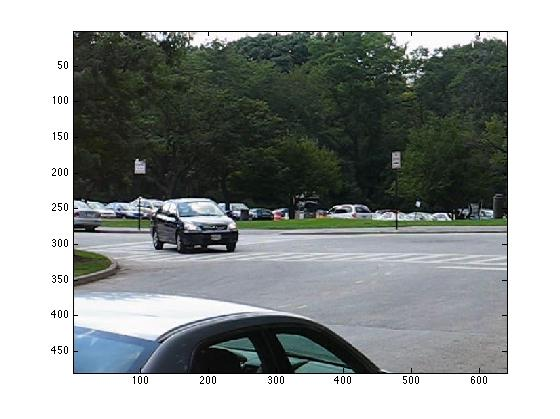
\includegraphics[scale=0.2]{figures/UnaryCostGT}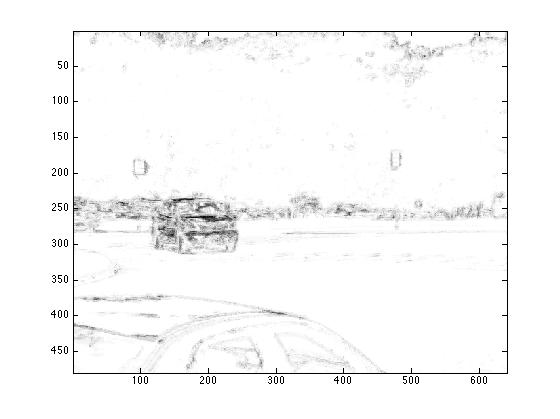
\includegraphics[scale=0.2]{figures/UnaryCost}\caption{Appearance Costs visualization : Low intensity represents low foreground cost
(object being tracked is upper car)}

\par\end{centering}

\end{figure}



\subsection{Finding flows given label assignments}


\subsection{Propogating labels}

\section{Complexity}

\begin{figure*}[t]
\begin{centering}
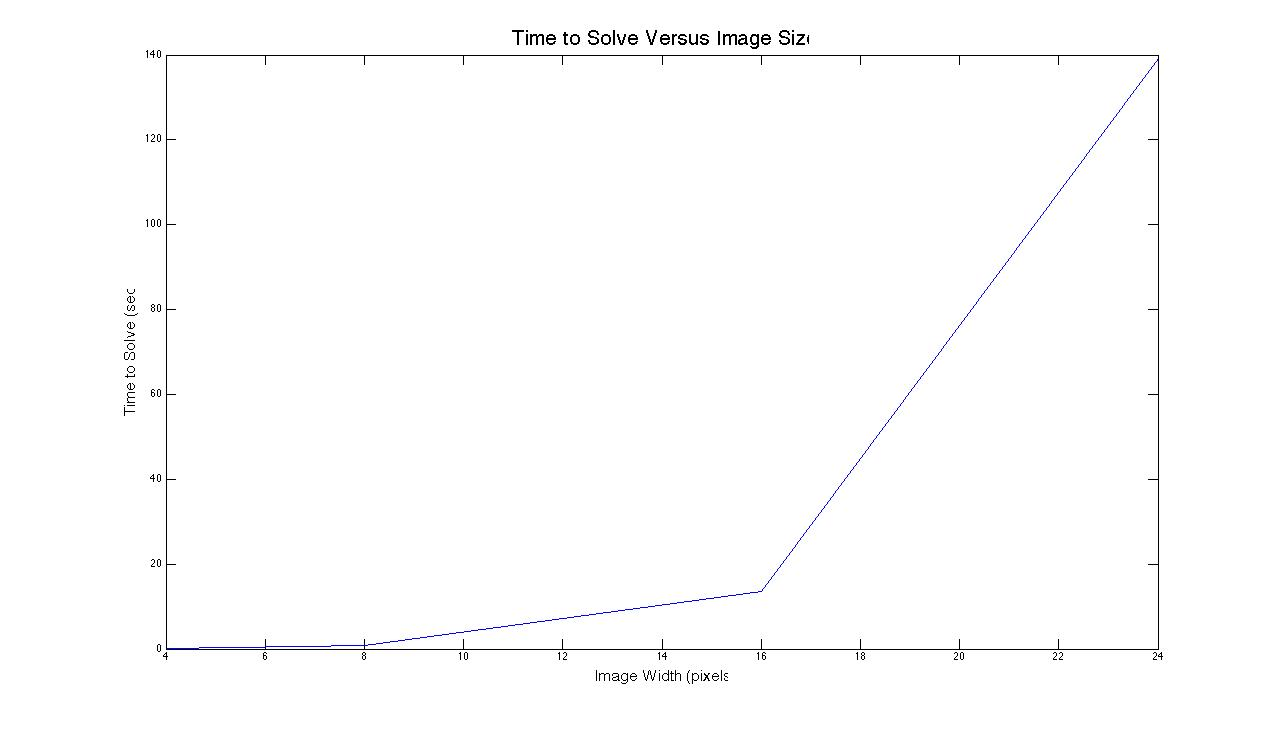
\includegraphics[scale=0.125]{figures/time_vs_imsize.jpg}
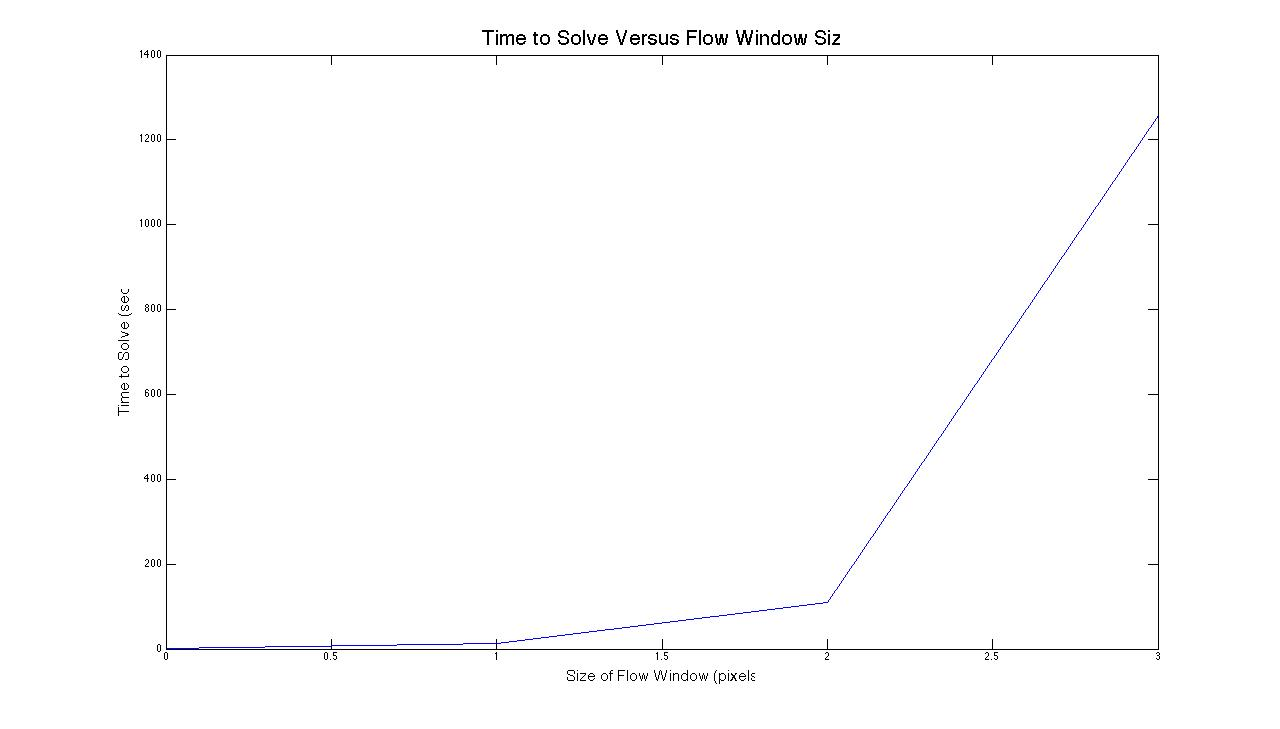
\includegraphics[scale=0.125]{figures/time_vs_window.jpg}
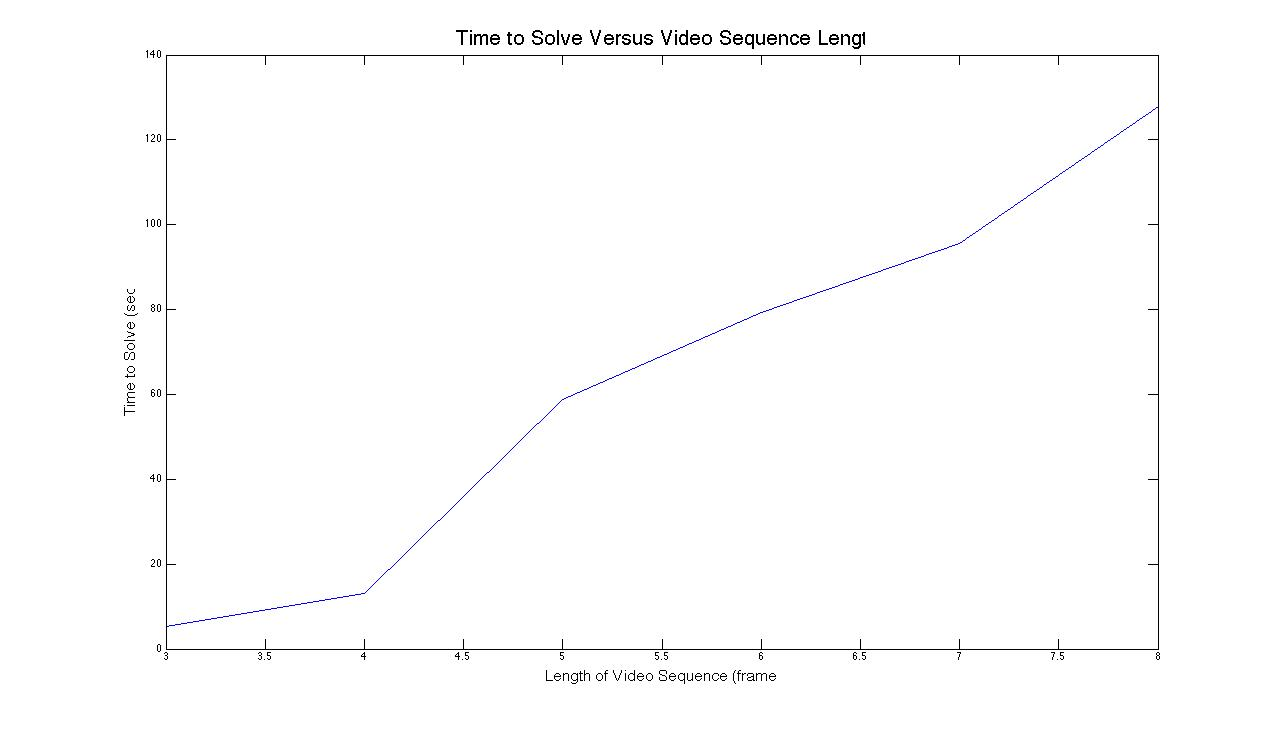
\includegraphics[scale=0.125]{figures/time_vs_length.jpg}
\caption{These graphs analyze the time to solve against (a) Image Dimension, 
(b) Window Size (temporal Neighborhood) and (c) Length of Sequence }
\par\end{centering}
\end{figure*}

Let $M$ x $N$ be the dimension of the video frames, $T$ be the lngth of the video sequence in frames, and $s$ be the width of the spatial neighborhood, and $w$ be the width of the temporal neighborhood. The original formulation of our problem has two variables: the labels $X$ and the edge weights $W$. There is a label for each pixel in the video sequence making $M N T$ label variables. There are $(2 w+1)^2$ weights for each pixel but no weights for the final frame, making $M N (T-1) (2 w + 1)^2$ weight variables. Therefore the original problem has a total of $M^2 N^2 T (T-1) (2 w + 1)^2$ variables. The momentum constraint has a term of the form $W_{ijt}^{ab} |c + \sum K W_{i^{'} j^{'} t+1} |$ which is non-convex, as can be shown by considering the trival example of $W_{ijt}^{ab} = 0.5$ and exactly one of the summed weights $= 0.5$ and testing the convexity condition. Thus the original problem is a quadratic program with a non-positive semidefinite quadratic term $Q$ and is NP-hard \cite{sahni1974computationally}.

Our primal decomposition method finds only an approximate solution to this problem by alternating between solving for the labels and weights using the Horn-Schunk first-order approximation of the imaging function as well as an approximation of the momentum term. With these changes both subproblems are convex.

First we consider the complexity of solving for the labels given the flows without the Horn-Schunk approximation. This problem has $M N T$ variables, but cannot be solved quickly in its raw form. For this reason we convert the problem to epigraph form, introducing $M N T$ new variables for spatial coherence and $M N T (2 w + 1)^2$ variables for temporal coherence. Therefore our total number of variables is $2 M N T + M N T (2 w + 1)^2$, which is typically dominated by the window term $N_{labels} \approx M N T (2 w + 1)^2)$. Since this is a linear integer programming problem it can be solved in order $O((M N T (2 w + 1)^2)^3)$ time. With the Horn-Schunk approximation the $(2 w + 1)^2$ term drops out, leading to $O((M N T)^3)$ solution time.

For solving the flows given the labels, the problem is considerably more difficult to solve with only the momentum approximation. There are $M N T (2 w + 1)^2$ variables to start with, but to put the problem in epigraph form we need to add $2 M N T (2 w + 1)^2 + 2 M N T + 2 M N T (2 w + 1)^2$ variables. This leads to a linear program which can be solved in 
$O((5 M N T (2 w + 1)^2)^3)$ time. With the Horn-Shunk approximation, all of our terms with $(2 w + 1)^2$ drop out, leading to $O((M N T)^3)$ time.

We empirically measured the time to find a solution along each of the dimensions $M, N, T$, and $w$. For simplicity we considered only square images. Figure ~\ref{fig:TimeVsIm} shows the time cost to solve versus the image dimension. We see that increasing the image dimension by a factor of 1.5 from 16x16 to 24x24 leads to a nearly 14x increase in solution time. Similarly in Figure ~\ref{fig:TimeVsLength} we see that the time to solve increases less dramatically, with the cost appearing almost linear. We suspect that this is because the problem size is small enough that the time to build the constraints actually dominates the solution time. Finally in Figure ~\ref{fig:TimeVsWin}, we see that the cost to solve increases dramatically with increased window size, as expected.

%
%\begin{center}
%	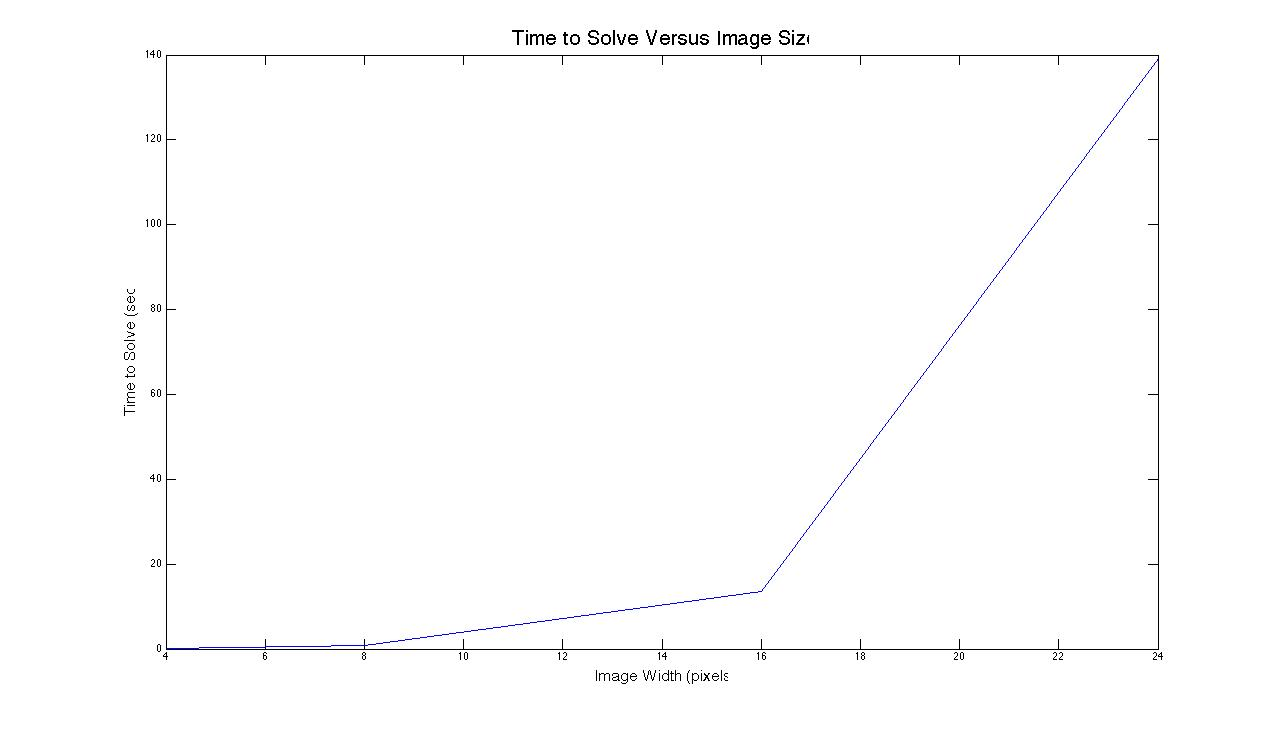
\includegraphics[width=0.45\textwidth, height=2in]{figures/time_vs_imsize.jpg}
%	\caption{Time to Solve versus Image Dimension}
%	\label{fig:TimeVsIm}
%\end{center}
%\begin{figure}[h]
%\begin{center}
%	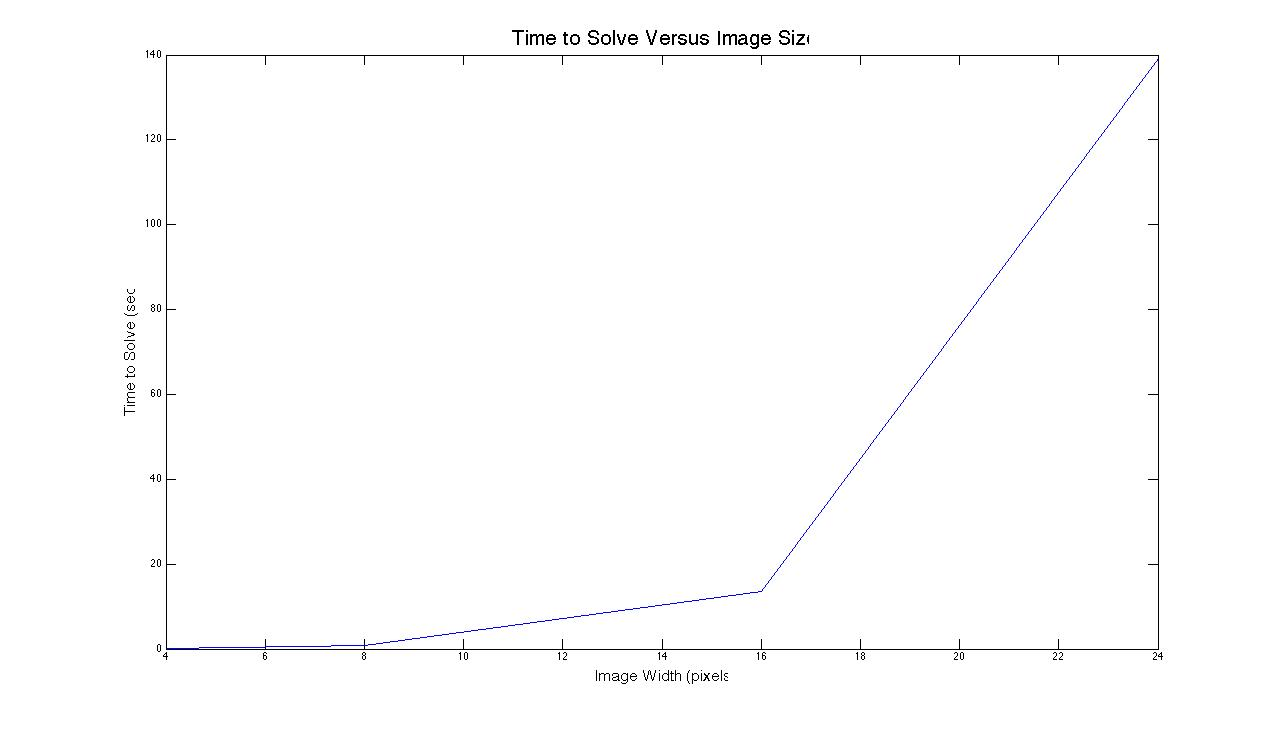
\includegraphics[width=0.45\textwidth, height=2in]{figures/time_vs_imsize.jpg}
%	\caption{Time to Solve versus Image Dimension}
%	\label{fig:TimeVsIm}
%\end{center}
%\end{figure}
%
%\begin{figure}[h]
%\begin{center}
%	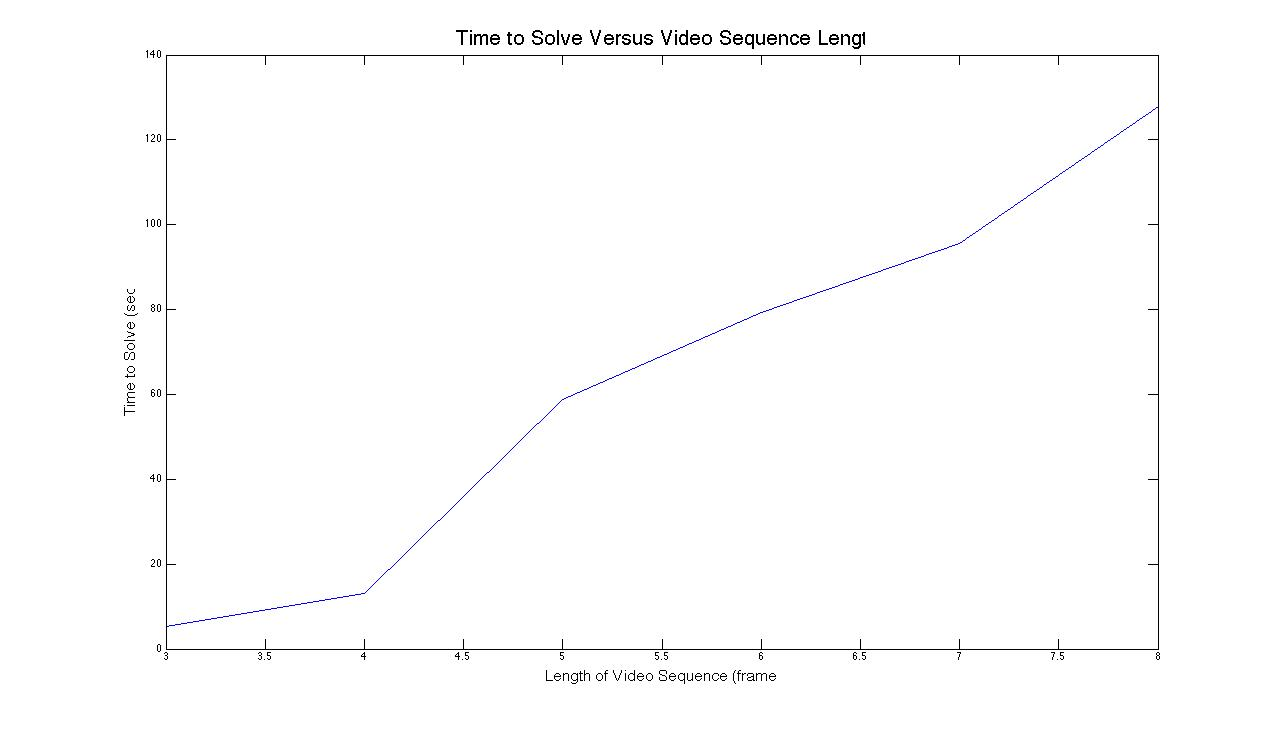
\includegraphics[width=0.45\textwidth, height=2in]{figures/time_vs_length.jpg}
%	\caption{Time to Solve versus Sequence Length}
%	\label{fig:TimeVsLength}
%\end{center}
%\end{figure}
%
%\begin{figure}[h]
%\begin{center}
%	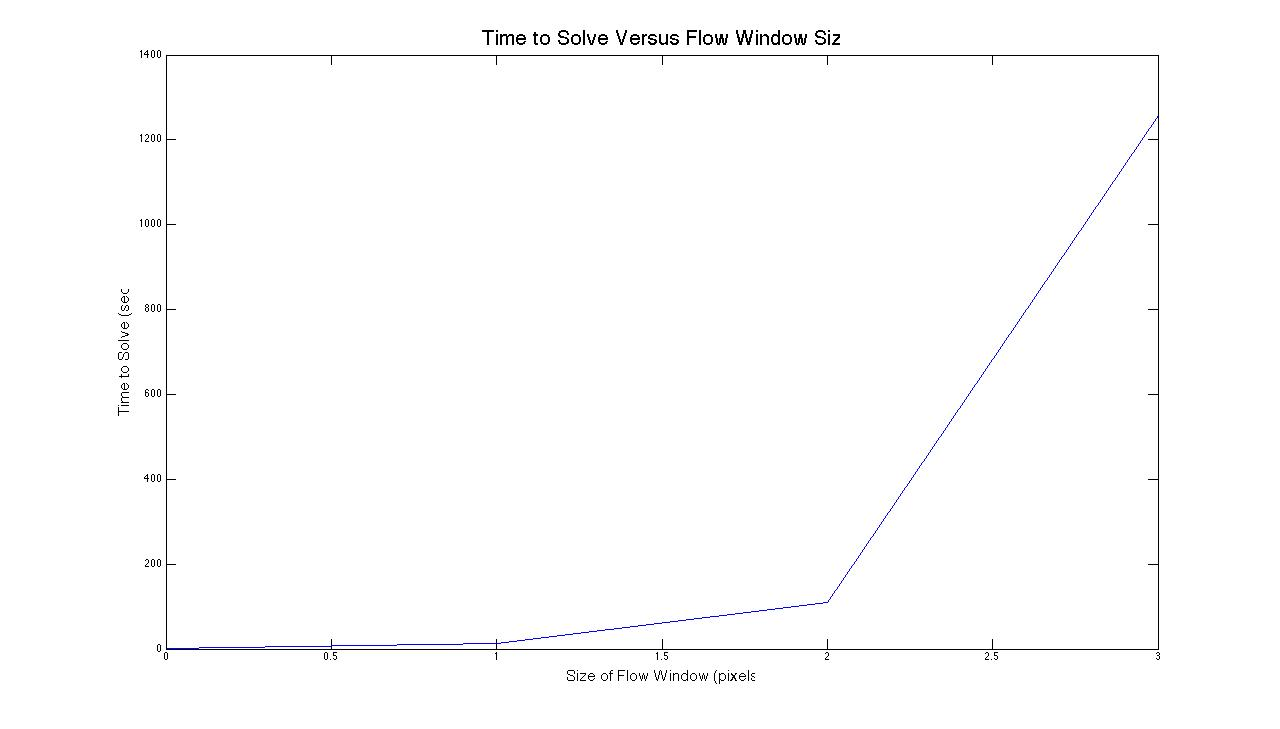
\includegraphics[width=0.45\textwidth, height=2in]{figures/time_vs_window.jpg}
%	\caption{Time to Solve versus Window Size}
%	\label{fig:TimeVsWin}
%\end{center}
%\end{figure}

\section{Experiments and Metrics}
\label{sec:Expt}
As presented in the model in Section~\ref{sec:ProbForm} we have a complete optimization
model with several integer variables for foreground-background labels.

We will test the performance of our solution on the 
Berkeley Motion Segmentation Dataset as provided by \cite{brox2010object}.
The dataset has 26 video sequences with pixel-accurate segmentation annotation of moving objects. A total of 189 frames are annotated.

We will evaluate results from our approach and compare the performance with that of \cite{Felzenszwalb2010b}, \cite{Komodakis2011a}
and \cite{brox2010object} on this dataset.

Furthermore multiple decoupling strategies will implementation and compared,
like decoupling time frames v/s decoupling in space. Finally a dual decomposition
method with also be explored and compared qualitatively with \cite{Komodakis2007a}.

We plan on completing the implementation in MATLAB with the use of CVX and CPLEX
optimization libraries.

\section{Conclusions and Future Work}
We were able to give a global optimization formulation for the problem of video segmentation where the objective was independently convex over two sets of variables. We used a block-coordinate descent method based solver for this global optimization problem and experimented with different formulations which resulted in different performances and accuracies. We observe that our algorithm is limited by the computational resources available and even though the global formulation would probably give better results, it still is a long way from being applied in practice because of the prohibhitive computational costs. We believe that the relaxations used in this work to arrive at a formulation of the problem as an $LP$ are general enough to capture the problem of video segmentation and can be leveraged in future work with better computational resources and hyper-parameter tuning to achieve state of the art results.


% Acknowledgements should only appear in the accepted version. 
%\section*{Acknowledgments} 
% 
%\textbf{Do not} include acknowledgements in the initial version of
%the paper submitted for blind review.
%
%If a paper is accepted, the final camera-ready version can (and
%probably should) include acknowledgements. In this case, please
%place such acknowledgements in an unnumbered section at the
%end of the paper. Typically, this will include thanks to reviewers
%who gave useful comments, to colleagues who contributed to the ideas, 
%and to funding agencies and corporate sponsors that provided financial 
%support.  


% In the unusual situation where you want a paper to appear in the
% references without citing it in the main text, use \nocite
%\nocite{langley00}

\bibliography{videoSeg}
\bibliographystyle{icml2014}

\end{document} 

